\section{Implementation and Evaluation}
\label{sec:count-sketch-implementation}

In order to facilitate easy implementation in a wide range of languages, including those from the functional programming paradigm, the operations of the count sketch are presented in the pseudocode as free-standing functions that operate on immutable input data structures without side effects.
The Java implementation takes full advantage of the object-oriented programming paradigm, however, and the corresponding methods are instance members of the mutable \lstinline{CountSketch} class, which implements the \lstinline{getFrequency(int)} query method of the \lstinline{FrequencySummary} interface.
Since the count sketch can accept both positive and negative items, the universe of items used in the implementation is defined to be a subset of the full range of the ubiquitous \num{32}~bit signed \lstinline{int} data type.
This allows the implementation to use the same item data type as that of the \lstinline{Fingerprint} (see \cref{sec:fingerprint-implementation}).
For a similar reason, the \lstinline{int} data type is also used to represent weights.
This means that the update methods of the \lstinline{Fingerprint} and the \lstinline{CountSketch} can share the signature \lstinline{update(int, int)}, which is declared in the \lstinline{MultisetSummary} interface.
The only constraint on the prime number is that it must be greater than the number of columns in the reduced array of the data.
Therefore, the prime chosen was the Mersenne prime \( 2^{31} - 1 \), which is the largest value that can be represented by the \lstinline{int} data type.
This allows up to \( 2^{31} - 2 \) columns in the array, although this many columns would never be used in practice as each row would be half the length of the entire universe of items.
Since multiple rows are required to return an accurate median, it would be more efficient in such a case to simply store the exact frequencies of the items.

The pairwise independent hash functions used in each row are implemented by the \lstinline{LinearHashFunction} class, which implements the \lstinline{apply(int)} method of the \lstinline{HashFunction} functional interface.
The constructor of the class takes a prime number \( p \) and a modulus, and draws a pair of linear and constant term coefficients from the interval \( \dataintegerinterval{1, p - 1} \).
For the hash functions that map items to positions in each row, the modulus is the number of columns.
For the discriminating hash functions, the modulus is two.
This produces a hash value in \( \dataset{0, 1} \), which is mapped to \( \dataset{-1, +1} \) via multiplication by two and subtraction of one.
One issue that arises in the implementation of the hash functions is that the remainder operator (\lstinline{\%}) computes the remainder according to \emph{truncated} division rather than \emph{Euclidean} division~\citep{o14}.
This means that it computes the least positive remainder of the integer division of the absolute value of the first argument by the absolute value of the second, and gives the result the sign of the first.
For positive dividends, this is equivalent to the Euclidean definition of the modulo operation, whereas for negative dividends, it produces negative remainders~\citep{boute92}.
Since the hash values are used as indices in an array, the modulo operations performed by the hash functions must return positive remainders.
The solution is to use the \lstinline{Math.floorMod} method, which computes the remainder according to Knuth's \emph{floored} division~\citep{knuth97,o14}.
Although this is not identical to the Euclidean definition, it does return positive remainders for positive divisors.
This replacement method need only be used for the first modulo operation, as it produces a positive dividend for the second modulo operation.

The initialization operation is implemented as a constructor that takes the number of rows and the number of columns to be used in the reduced array.
Since these sizes remain constant after initialization, the reduced array of data and the sequences of hash functions and estimates are implemented as native arrays rather than lists such as the \lstinline{ArrayList} from the Java collections framework.
The median method is implemented as a static method in the \lstinline{Math} utility class.
This sorts a given array and returns the middle element if the number of elements is odd, or the integer part of the arithmetic mean of the middle two elements if the number of elements is even.

The \lstinline{CountSketchAccumulator} class adapts the summary for use in Apache Spark (see \cref{subsec:introduction-structure-library}).
This allowed two types of test to be performed on the implementation of the count sketch.
The first was a test of the accuracy of its query operation.
The second was a test of the relationship between the size of a dataset and the time taken to construct its summary.
All tests were performed on a single machine using an Intel Core i5-9300H CPU with a base clock speed of \SI{2.40}{\giga\hertz}, four physical cores and eight logical processors, and \SI{8}{\gibi\byte} of RAM\@.
For information regarding how to run the tests, see \cref{app:repository}.

A failure in the accuracy of a count sketch occurs when the absolute error in its approximation of the multiplicity of an item exceeds an error bound expressed as a fraction of the \( L^{1} \)~norm \( \lnorm{1}{\mathvector{w}} \) of the vector of multiplicities of the multiset it summarizes.
The error bound considered in the accuracy test is the \( L^{1} \)~error bound given in \cref{subsec:count-sketch-analysis-accuracy}.
This states that a count sketch with \( m = \bigo{\ln (1 / \delta)} \) rows and \( n = \bigo{1 / \varepsilon} \) columns gives estimates whose absolute errors are at most \( \varepsilon \cdot \lnorm{1}{\mathvector{w}} \) with probability at least \( 1 - \delta \).
Since the failure bound \( \delta \) is determined by the number of rows \( m \), it can be verified empirically by varying the number of rows in the reduced array of the data.

Five series of accuracy tests were performed using the numbers of rows \num{3}, \num{5}, \num{7}, \num{9}, and~\num{11}.
Odd numbers of rows were chosen so as to allow the true median of the estimates of each item to be returned.
A fixed width of ten columns was used in all tests.
This corresponds to a relative error of \SI{10}{\percent} of the \( L^{1} \)~norm of the data.
To obtain a representative sample of results, each test was run \num{25}~times.
On each run, an artificial dataset was generated by drawing \( 2^{16} \) pairs of items and weights uniformly at random from the universe of items and the interval of weights, respectively.
This dataset size was chosen as it is large enough to warrant the use of a streaming algorithm, which offers a reduction in space requirements in exchange for less accurate results.
Conversely, it is not so large that the time and space consumed by the test could prevent other tests from being performed.
For a similar reason, a total of \( 2^{16} \) queries were performed on the count sketch constructed from each dataset.
The items chosen to be queried were distributed uniformly over the universe from which items were drawn.
Since the accuracy is independent of the size of this universe, the items could have been drawn from the full range of the \num{32}-bit signed integer data type used to represent items in the implementation.
However, since only \( 2^{16} \)~items would have been drawn from this range, and a different \( 2^{16} \)~items would have been queried, this would not have been a thorough test of the accuracy of the count sketch, as only one multiplicity at most in every \( 2^{16} \) would have been non-zero.
Instead, the universe was chosen to be \( \dataintegerinterval{-2^{16}, 2^{16} - 1} \).
This allowed for up to half of the items queried to have non-zero multiplicities in the dataset.

Although the weights contribute directly to the \( L^{1} \)~norm of the vector of multiplicities, they also contribute directly to the multiplicities and, to roughly the same extent, the absolute errors in their approximations.
Thus, the accuracy is independent of the size of the interval from which weights are drawn.
This allowed the weights to be drawn from a fixed interval \( \dataintegerinterval{-2^{7}, 2^{7} - 1} \), which can be represented as an \num{8}-bit signed integer.
This was small enough that in the unlikely case that all \( 2^{16} \)~items in the dataset were the same, and that their weights were either all the lower bound \( -2^{7} \) or all the upper bound \( 2^{7} - 1 \), the \num{32}-bit signed integer data type used to represent multiplicities in the implementation would not have overflowed.

Using the Apache~Spark stream processing framework, each dataset was read as input and passed one pair at a time to a \lstinline{CountSketchAccumulator}, which constructed a \lstinline{CountSketch} of the multiset.
Apache~Spark was run using one worker thread for each of the eight logical processors of the test machine.
By running the summary construction in parallel, the correctness of the merge operation was also verified.
The summary was queried for approximations of the multiplicities of \( 2^{16} \) items.
Each approximation was compared to the corresponding true multiplicity in the dataset, and its absolute error was calculated.
If this exceeded the expected error bound \( \varepsilon \cdot \lnorm{1}{\mathvector{w}} \), the query was considered to have failed.
Over all the queries of all the runs that used a given number rows, the proportion of failures was calculated.
If this was less than the corresponding failure bound \( \delta \), the series of tests was considered to have passed.

\begin{table}
  \centering
  \caption{Results of the accuracy tests}
  \label{tab:count-sketch-implementation-accuracy}
  \begin{tabular}{
  S[
    table-alignment = right,
    table-format = 2,
  ]
  S[
    round-mode = figures,
    round-precision = 3,
    table-alignment = right,
    table-format = 1.2e-1,
  ]
  S[
    table-alignment = right,
    table-format = 1,
  ]
}
  \toprule
  {Rows} & \multicolumn{2}{c}{Failure proportion} \\
  \cmidrule{2-3}
  & {Upper bound} & {Observation} \\
  \midrule
  3 & 0.04978706837 & 0 \\
  5 & 6.737946999e-3 & 0 \\
  7 & 9.118819656e-4 & 0 \\
  9 & 1.234098041e-4 & 0 \\
  11 & 1.670170079e-5 & 0 \\
  \bottomrule
\end{tabular}
%
\end{table}

The results of all \num{25}~runs of each of the five accuracy tests are presented in \cref{tab:count-sketch-implementation-accuracy}.
This includes the number of rows in the reduced array of the data, the upper bound on the probability of exceeding the expected error bound, and the proportion of failures observed.
Every query passed on every run of every test.
This provides an empirical verification of the correctness of both the design of the count sketch, and the upper bounds on the probabilities of errors and failures.
It should be noted that the failure bound of the last test corresponds to odds of approximately one in \num{60}~thousand.
As with the fingerprint summary, performing this many runs was deemed both infeasible and unnecessary (see \cref{sec:fingerprint-implementation}).
The total of \num{125}~runs was sufficient to show that the probability of a failure is low, even for as few as three rows.

The relationship between the size of a dataset and the time taken to construct its summary was tested via performance tests.
Five series of performance tests were performed using dataset sizes of \( 2^{8} \), \( 2^{12} \), \( 2^{16} \), \( 2^{20} \) and~\( 2^{24} \).
For each of the five series, \num{26}~artificial datasets were generated by drawing the corresponding numbers of pairs of items and weights, in the same manner as for the accuracy tests.
Since only the size of the data was varied for these tests, the items were drawn from the full range of the \num{32}-bit signed integer data type, and the weights were drawn from the arbitrary fixed interval \( \dataintegerinterval{-2^{7}, 2^{7} - 1} \).
After all \num{26}~datasets had been generated, the construction of the \lstinline{CountSketch} of each dataset was timed using only a single worker thread.
The execution time was calculated as the positive difference between the values returned by calls to \lstinline{System.nanoTime()} immediately before and immediately after the construction.
Although this method gives nanosecond precision by querying the most precise available system timer~\citep{o14}, it does not necessarily give nanosecond accuracy, since there is no guarantee regarding the frequency with which this value is updated~\citep{lambert08}.
Nevertheless, it can be assumed that, on average, it is accurate to within hundreds of nanoseconds~\citep{kuperberg09}.
The first run of each series of tests was discarded, as this run `warms up' the test architecture by loading process data into memory and, therefore, encounters page faults and cache misses that should not be considered a feature of normal operation~\citep{luo04}.
The median of the remaining \num{25}~runs was calculated.
Since the execution time can vary greatly due to the presence of other processes, the median is more suitable than the mean as a representation of the typical execution time, as it is not so easily skewed by outliers, and remains meaningful after normalization~\citep{fleming86}.
A sixth series of tests was performed using a dataset containing only a single item--weight pair.
The median execution time of this series was taken as an approximation of the fixed overhead associated with starting the test and initializing the summary.
This was subtracted from the median execution times of the other series of tests in order to normalize them such that they represent only the time taken to update the summary for each item--weight pair in the corresponding dataset.

\begin{table}
  \centering
  \caption{Results of the performance tests}
  \label{tab:count-sketch-implementation-performance}
  \begin{tabular}{
  S[
    table-alignment = right,
    table-format = 8,
  ]
  S[
    table-alignment = right,
    table-format = 11,
  ]
  S[
    table-alignment = right,
    table-format = 11,
  ]
}
  \toprule
  {Dataset size} & \multicolumn{2}{c}{Execution time / \si{\nano\second}} \\
  \cmidrule{2-3}
  & {Median} & {Normalized} \\
  \midrule
  1 & 28351887 & 0 \\
  256 & 30062300 & 1710413 \\
  4096 & 51011800 & 22659913 \\
  65536 & 327077500 & 298725613 \\
  1048576 & 4751193500 & 4722841613 \\
  16777216 & 79928476900 & 79900125013 \\
  \bottomrule
\end{tabular}
%
\end{table}

\begin{figure}
  \centering
  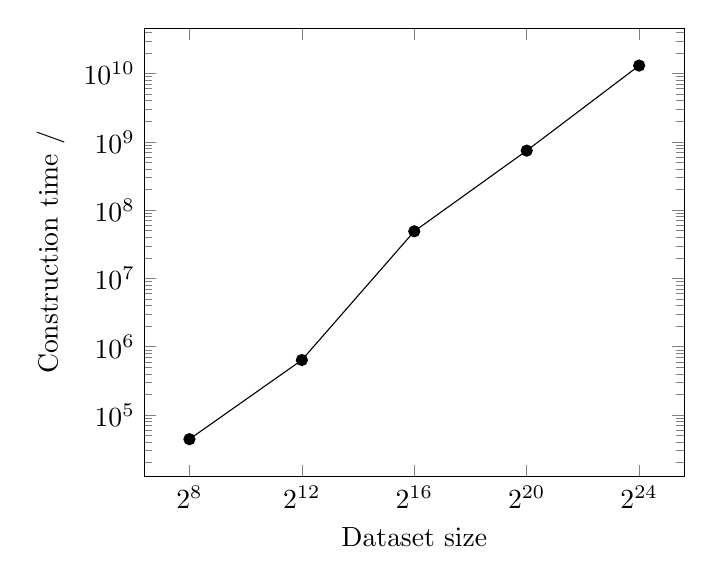
\begin{tikzpicture}
  \begin{loglogaxis}[
    log basis x = 2,
    log basis y = 10,
    xlabel = {Dataset size},
    xtick = {2^8, 2^12, 2^16, 2^20, 2^24},
    ylabel = {\text{Construction time} / \si{\nano\second}},
  ]
    \addplot [mark=*,black] coordinates {
      (256, 44277)
      (4096, 638777)
      (65536, 49027776)
      (1048576, 743982676)
      (16777216, 13091972575)
    };
  \end{loglogaxis}
\end{tikzpicture}
%
  \caption{Relationship between dataset size and summary construction time}
  \label{fig:count-sketch-implementation-performance}
\end{figure}

The results of all \num{25}~runs of each of the five performance tests are presented in \cref{tab:count-sketch-implementation-performance}, and the relationship between the size of a dataset and the time taken to construct its summary is shown in \cref{fig:count-sketch-implementation-performance}.
This relationship appears to be linear, which agrees with the analysis given in \cref{subsec:count-sketch-analysis-complexity}.
Since the update operation has constant time complexity per update in the size of the data---not to be confused with its linear time complexity in the number of rows---and one update is performed for every item--weight pair in the dataset, the time complexity associated with performing all the updates given in a dataset is linear in the size of the dataset.
